\section{Sampling the MDM in the discrete and the continuum}
If we forget about the directions of the edges, the resulting undirected graph is supercritical, and, with high probability, the graph contains a unique giant component with surplus going to infinity as $n\to \infty$ (see e.g. \cite{molloyCriticalPointRandom1995}, \cite{Molloy1998}, \cite{Janson2009} for a discussion of the phase transition in the undirected configuration model). This suggests that if we do not dismiss a large amount of edges, we will not be able to study the digraph in enough detail to find a metric space scaling limit of the strongly connected components. Therefore, we will not try to sample the entire digraph, but focus on the information that we need to find the strongly connected components. We start by studying the discrete graph model, with the goal of identifying which edges can be part of a strongly connected components, and how to sample them. In Subsubsection \ref{subsubsec.defcandidates}, we establish necessary conditions for an edge to be part of a strongly connected component. The result implies that we only need to study the out-forest, and a small subset of the surplus edges, which we call \emph{candidates}. In Subsubsections \ref{subsubsec.samplingoutforest} and \ref{subsubsec.samplecandidates} we study the law of the out-forest and the candidates respectively, and we define a procedure to sample both. This yields a sequence of directed multigraphs with edge lengths that the strongly connected components are embedded in.  
In Subsection \ref{subsec.limitobject}, we define the continuous counterpart of the sampling procedure. The resulting object will the limit under rescaling of the sequence of directed multigraphs with edge lengths that the strongly connected components are embedded in that was constructed in Subsubsections \ref{subsubsec.samplingoutforest} and \ref{subsubsec.samplecandidates}. 
\subsection{The discrete case}\label{subsec.discrete}
We will discuss the different type of edges that we can encounter in the exploration. By slight abuse of notation, we call the purple vertex that corresponds to a surplus edge its tail.

\subsubsection{Necessary conditions for an edge to be part of an SCC}\label{subsubsec.defcandidates}
Amongst the surplus edges, \emph{ancestral surplus edges}, which are surplus edges that point from a vertex to one of its ancestors, play a special rôle. All other surplus edges are called non-ancestral. This is illustrated in Figure \ref{subfigure.typesofsurplusedges}. In Figure \ref{subfigure.sccinexample} we show how surplus edges affect the structure of the strongly connected components. This is the content of Lemma \ref{lemma.whatispartofscc}.
\begin{lemma}\label{lemma.whatispartofscc}
The following facts hold for strongly connected components. 
\begin{enumerate}
\item \label{item.factsonsccs1}The vertices of a strongly component are contained in one of the components of $(\hat{F}_n(k),k\geq 1)$. 
\item \label{item.factsonsccs2} Ancestral surplus edges are always part of a strongly connected component.
\item \label{item.factsonsccs4} A non-ancestral surplus edge is only part of a strongly connected component if its head is an ancestor of the tail of a surplus edge that is part of a strongly connected component.
\item \label{item.factsonsccs4andabit} An edge in $(\hat{F}_n(k),k\geq 1)$ is only part of a strongly connected component if its head is an ancestor of the tail of a a surplus edge that is part of a strongly connected component.
\item \label{item.factsonsccs5} For any non-trivial strongly connected component, the first surplus edge of the SCC that is explored is an ancestral surplus edge, and a component of  $(\hat{F}_n(k),k\geq 1)$ contains a strongly connected component if and only if it contains an ancestral surplus edge.
\end{enumerate}
\end{lemma}
\begin{proof}
We start with \ref{item.factsonsccs1}. Let $v$ and $w$ be two vertices in the same strongly connected component. Without loss of generality, $v$ is explored first in depth-first order in the out-direction. Since $v$ and $w$ are part of the same strongly connected component, we know that there is a path from $v$ to $w$ in the out-direction. This implies that $w$ will be part of the out-subtree consisting of the descendants of $v$. This implies that they are part of the same component of $(\hat{F}_n(k),k\geq 1)$. \\
To prove \ref{item.factsonsccs2}, suppose there is an ancestral surplus edge from $v$ to $w$. This implies that $w$ is an ancestor of $v$ in an out-component, which implies that there is a path from $w$ to $v$ as well. It follows that $w$ and $v$ are in the same strongly connected component and that the ancestral surplus edge from $v$ to $w$ is in this strongly connected component as well. \\
To prove \ref{item.factsonsccs4}, suppose we sample a non-ancestral surplus edge from $v$ to $w$ that is part of a strongly connected component. Then, by \ref{item.factsonsccs2}, there is a path from $w$ to $v$ present at the time of sampling $(v,w)$. Let $(x,y)$ be the first surplus edge on this path. This implies that $(x,y)$ is in the same strongly connected component as $v$ and $w$. Moreover, the path from $w$ to $x$ consists of edges in the out-forest, $x$ is a descendant of $w$.\\
Next, for \ref{item.factsonsccs4andabit}, suppose $(v,w)$ is an edge of $(\hat{F}_n(k),k\geq 1)$ that is part of a strongly connected component. This means that there is a path from $w$ to $v$. Let $(x,y)$ be the first edge on this path such that $y$ is not a descendant of $w$. Then, $(x,y)$ is a surplus edge that is part of the same strongly connected component as $v$ and $w$, and $(v,w)$ is on the path from the root to $x$. \\
Finally, \ref{item.factsonsccs2} and \ref{item.factsonsccs4} imply \ref{item.factsonsccs5}. 
\end{proof}

Lemma \ref{lemma.whatispartofscc} motivates the following definition.
\begin{definition}\label{def.candidate}
A surplus edge is a \emph{candidate} if either
\begin{itemize}
    \item It is an ancestral surplus edge, or
    \item One of the descendants of its head is the tail of a candidate.
\end{itemize}
\end{definition}
The following corollary is at the core of our strategy to study the strongly connected components.
\begin{corollary}\label{cor.edgesinSCCs}
All edges that are part of a strongly connected component are either a candidate, or are contained in the subforest of $(\hat{F}_n(k),k\geq 1)$ that is spanned by the tails of candidates and the roots of the out-components.
\end{corollary}
\begin{proof}
This follows from Definition \ref{def.candidate} and parts \ref{item.factsonsccs1}, \ref{cond.excursions2}, \ref{item.factsonsccs4} and \ref{item.factsonsccs5} of Lemma \ref{lemma.whatispartofscc}.
\end{proof}
\begin{figure}
\centering
\begin{subfigure}{0.7\textwidth}
 \centering
    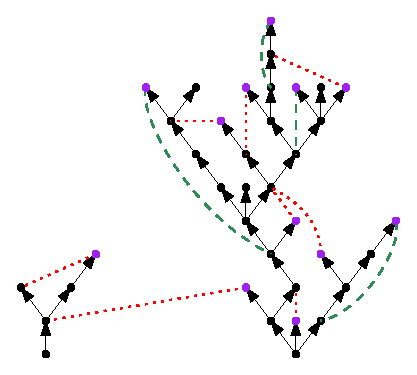
\includegraphics[width=0.7\linewidth]{Content/Pictures/types_of_surplus_edges.eps}
    \caption{This figure illustrates an example of a depth-first exploration of two out-components with the different type of surplus edges highlighted. The ancestral surplus edges (green dashed) point from a vertex $v$ to one of its ancestors. They are always part of a strongly connected component. The other surplus edges are depicted as red dotted lines.}
    \label{subfigure.typesofsurplusedges} 
\end{subfigure}\\
\begin{subfigure}{0.7\textwidth}
  \centering
  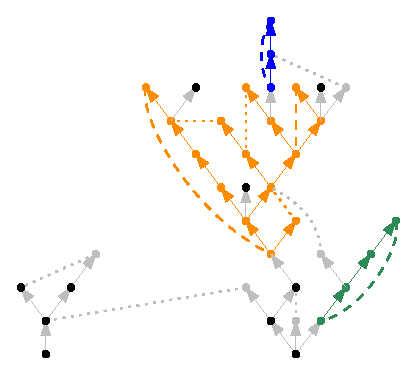
\includegraphics[width=0.7\linewidth]{Content/Pictures/sccs_in_example.eps}
  \caption{The non-trivial strongly connected components embedded in the components of the out-forest are depicted in orange, blue and green. The trivial strongly connected components are black. The grey edges are not part of a strongly connected component, and the grey vertices correspond to purple leaves that are not part of a strongly connected component.}
    \label{subfigure.sccinexample}
\end{subfigure}
\caption{We illustrate the different types of surplus edges and how they affect the structure of the strongly connected components.}
\end{figure}

Corollary \ref{cor.edgesinSCCs} implies that for every purple vertex, we only need to know whether it is a candidate, and if so, where its head is. 
\subsubsection{Sampling the out-forest}\label{subsubsec.samplingoutforest}
This subsubsection discusses how to obtain the out-forest conditional on the order in which the vertices are discovered. We will study the law of the degrees in order of discovery in Subsection \ref{subsec.measurechange}. Informally, the out-forest is obtained in the following way. Suppose the degrees in order of discovery are given by $(\mathbf{\hat{D}}_{n,1},\dots,\mathbf{\hat{D}}_{n,n})$. Up to time step $k$, suppose we have added the vertices corresponding to the first $m\leq k$ elements of  $(\mathbf{\hat{D}}_{n,1},\dots,\mathbf{\hat{D}}_{n,n})$ to the forest. We call these vertices \emph{discovered}. Then, at time $k+1$,
\begin{enumerate}
    \item If we have finished a component of the out-forest, let the next out-component have a root with out-degree $\hat{D}_{n,m+1}^+$. 
    \item Otherwise,
    \begin{enumerate}\item With probability proportional to the total in-degree of the undiscovered vertices, i.e. $\sum_{i={m+1}}^n \hat{D}_{n,i}^-$, let the next vertex in depth-first order be a black vertex with out-degree $\hat{D}_{n,m+1}^+$.
    \item With probability proportional to the unpaired in-half-edges of the $l$ discovered vertices, let the next vertex in depth-first order be a purple leaf, and reduce the number of unpaired in-edges of the $l$ discovered vertices by $1$.
\end{enumerate}
\end{enumerate}
We make this rigourous in the following lemma.
\begin{lemma}\label{lemma.sampleoutforest}
Suppose the sequence of degrees in order of discovery $(\hat{D}^n_1,\dots,\hat{D}^n_n)$ is given. Suppose, for $1\leq l\leq k$, that up to time $l$, $\hat{P}_n(l)$ surplus edges have been sampled. Then, $$\left(\hat{S}^+_n(l),1\leq l\leq k \right):=\left(\sum_{i=1}^{l-\hat{P}_n(l)}\hat{D}^+_{n,i}-l,1\leq l\leq k\right)$$ is the \L ukasiewicz path of the out-forest up to time $k$. Moreover, for $$\left(\hat{I}^+_n(l),1\leq l\leq k\right):=\left(\min\left\{\hat{S}^+_n(m):1\leq m \leq l\right\},1\leq l \leq k \right),$$
define 
$$\left(\hat{S}^-_n(l),1\leq l \leq k\right):=\left(\sum_{i=1}^{l-\hat{P}_n(l)}\hat{D}^-_{n,i}-l-\hat{I}^+_n(l)+1,1\leq l\leq k\right),$$
so that $\hat{S}^-_n(k)$ is equal to the number of unpaired in-half-edges of discovered vertices at time $k$. Then, the probability that we sample a surplus edge at the $(k+1)^{th}$ time step is given by
$$\frac{\hat{S}^-_n(k+1)}{\sum_{i=1}^n D^-_i-k-\hat{I}^+_n(k)+1}\one_{\left\{\hat{I}^+_n(k)=\hat{I}^+_n(k-1)\right\}}.$$
Therefore, we do not need to know the position of the heads of the surplus edges to sample the out-forest.
\end{lemma}
\begin{proof}
Note that if up to time $k$, $\hat{P}_n(k)$ surplus edges have been sampled, this implies that $k-\hat{P}_n(k)$ vertices have been discovered. Thus, up to time $k$, the out-forest contains $\hat{P}_n(k)$ purple leaves, and black vertices with degrees $(\hat{D}^+_{n,1},\dots,\hat{D}^+_{n,k-\hat{P}_n(k)})$, so by definition of the \L ukasiewicz path, its value is indeed equal to $\hat{S}^-_n(k)$ at time $k$. Moreover, up to time $k$, the total in-degree of the discovered vertices is equal to $\sum_{i=1}^{k-\hat{P}_n(k)}\hat{D}^-_{n,i}$. At every time step, we pair $1$ in-half-edge of a discovered vertex, unless we start a new component. $-\hat{I}^+_n(k)$ corresponds to the number of out-components that are finished up to time $k$, so the total number of unpaired in-half-edges of discovered vertices at time $k$ is equal to $\hat{S}^-_n(k)$. By the same reasoning, the total number of unpaired in-half-edges is equal to $\sum_{i=1}^n D^-_i-k-\hat{I}^+_n(k)+1$. The probability of sampling a surplus edge follows. We note that this probability does not depend on the position of the heads of the surplus edges, which implies that we can sample the out-forest without this information.
\end{proof}
\subsubsection{Sampling the candidates}\label{subsubsec.samplecandidates}
We will now study the law of the candidates conditional on $(\hat{F}_n(k),k\geq 1)$. As before, for each $k$, let $\hat{P}_n(k)$ denote the number of purple vertices amongst the first $k$ vertices in the out-forest, and let $\hat{S}^-(k)$ denote the number of unpaired in-half-edges of discovered vertices at time $k$. We will first identify the tails of the candidates amongst the purple vertices, and then we will sample the position of their heads. \\
If the vertex visited at time $k$ is purple, the head of the corresponding surplus edge is a uniform pick from the $\hat{S}^-(k)$ unpaired in-half-edges of discovered vertices at time $k$. Therefore, the probability that a purple vertex visited at time $k$ corresponds to an ancestral surplus edge is given by the number of unpaired in-edges on its path to the root divided by $\hat{S}^-(k)$. This implies that to understand the law of the position of ancestral surplus edges, we need to understand where the unpaired in-edges are. \\
We will study this by modifying the edge lengths in the tree: for a vertex $v$ with in-degree $m$, the edges connecting it to its children will have length $m-1$ (unless $v$ is the root of an out-component, then the edges connecting to its children will have length $m$). The height of vertex $w$ in this forest with edge lengths corresponds to the number of in-half-edges that can be used to form an ancestral surplus edge with tail $w$. We add lengths to all edges in $(\hat{F}_n(k),k\geq 1)$ and call the resulting forest with edge lengths $(\hat{F}^\ell(k),k\geq 1)$. Denote the height process of $(\hat{F}^\ell(k),k\geq 1)$ by $(\hat{H}_n^\ell(k),k\geq 1)$. \\
Recall that the first candidate in any component of $(\hat{F}_n(k),k\geq 1)$ is an ancestral surplus edge. The following lemma illustrates the importance of $\hat{H}^\ell$ in finding the first ancestral surplus edges in the out-components.

\begin{lemma}\label{lemma.probancestral}
Consider the exploration of $(\hat{F}_n(k),k\geq 1)$ at time $k$. If no ancestral surplus edge has been sampled in the current component, then the probability that $k$ is the tail of an ancestral surplus edge is given by 
$$a_k=\frac{\hat{H}^\ell(k)}{\hat{S}_n^-(k)}\one_{\{\hat{P}_n(k)-\hat{P}_n(k-1)=1\}}.$$
This event is independent of the position of the heads of the surplus edges that were found before time $k$.
% If $k$ is the tail of an ancestral surplus edge, then the position of the end point $Y$ has the following law. Let $U$ be uniform on $[0,\hat{H}^\ell(k)]$. Then, let $Y_k$ be the height of youngest ancestor $l$ of $k$ such that $H^{\ell}(l)<U$. 
\end{lemma}
\begin{proof}
We claim that if no ancestral surplus edge has been sampled in the current component, none of the ancestors of $k$ are the head of a surplus edge. Indeed, for $x$ an ancestor of $k$, all vertices that are visited since the discovery of $x$ up to time $k$ are descendants of $x$, because $(\hat{F}_n(k),k\geq 1)$ is explored in a depth-first manner. Therefore, any surplus edge with head $x$ sampled up to time $k$ is ancestral. This implies that for $d^-$ the in-degree of $x$, the number of unpaired in-half-edges of $x$ at time $k$ is equal to $d^--1$ (unless $x$ is the root of the out-component, in which case it has $d^-$ unpaired in-half-edges).

Therefore, the number of unpaired in-half-edges corresponding to ancestors of $k$ is equal to $H^\ell(k)$. Moreover, note that, by definition of the purple vertices, $k$ is the tail of a surplus edge if and only if $k$ is purple, i.e. if and only if $\hat{P}_n(k)-\hat{P}_n(k-1)=1$. In that case, the probability that it connects to given unpaired in-half-edge of a visited vertex is equal to $1/\hat{S}_n^-(k)$. The stated probability follows. The independence on the position of the heads of earlier surplus edges is immediate.
\end{proof}

We now illustrate how to find the other candidates in a component of $(\hat{F}_n(k),k\geq 1)$. 
\begin{lemma}\label{lemma.samplecandidates}
Let $T^n_{l_n}$ be a component of $(\hat{F}_n(k),k\geq 1)$ with root $l_n+1$ and component length $\sigma_n$. Suppose the first ancestral surplus edge in $T^n_{l_n}$ corresponds to purple vertex $V^n_1\in [l_n+2,l_n+\sigma_n]$. Let $V^n_1<k\leq l_n+\sigma_n$, and suppose the candidates found up to time $k$ are given by $V^n_1,\dots,V^n_m$. Let $T^{n,\text{mk}}_k$ be the subtree of $T^n_{l_n}$ spanned by $\{l_n+1,V^n_1,\dots,V^n_m,k\}$, and let $\ell(T^{n,\text{mk}}_k)$ be its total length with edge lengths as defined by $(\hat{H}^\ell(m),m\in [l_n+1,l_n+\sigma_n])$. Then, the probability that $k$ is a candidate is given by 
$$\frac{\ell\left(T^{n,\text{mk}}_k\right)-l}{\hat{S}^-(k)}\one_{\{\hat{P}_n(k)=\hat{P}_n(k-1)+1\}}.$$
\end{lemma}
\begin{proof}
Note that if $k$ is purple, it gets paired to a uniform pick from the $\hat{S}^-(k)$ unpaired in-half-edges of discovered vertices. By Definition \ref{def.candidate}, in that case, $k$ is a candidate if and only if its head is in $T^{n,\text{mk}}_k$. Observe that $\ell\left(T^{n,\text{mk}}_k\right)$ is equal to the number of in-half-edges of $T_{k}$ that can be used to form surplus edges. By the definition of a candidate, exactly $m$ of those have been paired: one for each element in $\{V^n_1,\dots,V^n_m\}$. This implies that $\ell\left(T^{n,\text{mk}}_k\right)-m$ of the $\hat{S}^-(k)$ options will cause $k$ to be a candidate.
\end{proof}

Note that the probability that a purple vertex corresponds to a candidate only depends on the out-forest and the number of candidates that have been found in the component so far. The position of the heads of the candidates can be found as follows.
\begin{lemma}\label{lemma.sampleheadcandidates}
Let $T^n_{l_n}$ be a component of $(\hat{F}_n(k),k\geq 1)$ with root $l_n+1$ and component length $\sigma_n$. Suppose its candidates are given by $\{V^n_1,\dots,V^n_{N_n}\}$. Then, for $1\leq i\leq {N_n}$, suppose the heads of the surplus edges corresponding to $V^n_1,\dots,V^n_{i-1}$ are given by $W_1^n,\dots,W^n_{i-1}$ respectively. Then, the in-half-edge that $V^n_{i}$ gets paired to is a uniform pick from the $$\ell\left(T^{n,\text{mk}}_{V^n_i}\right)-(i-1)$$ unpaired in-half-edges of $T^{n,\text{mk}}_{V^n_i}$ that remain. Call the corresponding vertex $W^n_i$.
\end{lemma}
\begin{proof}
Given that $V^n_{i}$ is a candidate, its head will be in $T^{n,\text{mk}}_{V^n_i}$. Then, the distribution follows.
\end{proof}

Lemmas \ref{lemma.sampleoutforest}, \ref{lemma.probancestral}, \ref{lemma.samplecandidates}, and \ref{lemma.sampleheadcandidates} justify the following sampling procedure.
\begin{enumerate}
    \item Sample the out-forest $(\hat{F}_n(k),k\geq 1)$.
    \item Fix $T>0$ and define a counting process $(A_n(k),k\leq \lfloor Tn^{2/3}\rfloor)$, with the probability of an increment at time $k$ given by $$a_k=\frac{\hat{H}_n^\ell(k)}{\hat{S}_n^-(k)}\one_{\{\hat{P}_n(k)-\hat{P}_n(k-1)=1\}}.$$
    \item For $i\geq 1$, set $X_i^n=\min\{k:A_n(k)=i\}$. Define
\begin{align*}L_i^n&=\min\left\{k\geq 1:\hat{S}^{+}_n(k)=\min\{\hat{S}^{+}_n(l):l\leq X_i^n\}\right\}\text{ for }i\geq 1\\
\Sigma_i^n&=\min\left\{k \geq 1: \min\left\{\hat{S}^{+}_n(l):l\leq L_i^n+k\right\} < \min\left\{\hat{S}^{+}_n(l):l\leq X_i^n\right\}\right\}\text{ for }i\geq 1,
\end{align*}
so that for each $i\geq 1$, $\left(\hat{S}^+(k),k\in [L_i^n+1,L_i^n+\Sigma_i^n]\right)$ encodes the out-tree containing $X_i^n$. For each $(l_n,\sigma_n)\in \{(L_i^n,\Sigma_i^n)\}$, let $T^n_{l_n}$ be the tree in $(\hat{F}_n(k),k\geq 1)$ with root $l_n+1$, and do the following.
    \begin{enumerate}
    \item \label{item.procedure3} Set $V_1^n=\min\{m\geq 1:A_n(m)=A_n(g)+1\}$, and find the other candidates $\{V_2^n,\dots ,V_{N_n}^n\}$ according to the procedure described in the statement of Lemma \ref{lemma.samplecandidates}.
    \item \label{item.procedure4} For $V_1^n,\dots, V_{N_n}^n$, sample their heads $W_1^n,\dots ,W_{N_n}^n$ respectively according to the procedure described in the statement of Lemma \ref{lemma.sampleheadcandidates}.
    \item Let $T^{n,\text{mk}}(l_n)$ be the subtree of $T^n_{l_n}$ spanned by $\{l_n+1,V_1^n,\dots ,V_{N_n}^n\}$, say $V_i^n\sim W_i^n$ for each $1\leq i\leq N_n$, and set $M^n_{l_n}:=T^{n,\text{mk}}(l_n)/\sim$, which we note is a directed graph with surplus $N_n$. 
\end{enumerate}
\end{enumerate}
Then, all strongly connected components of $\vec{G}_n(\nu)$ of which the first candidate is sampled before time $\lfloor Tn^{2/3}\rfloor$ are subgraphs of $\left\{M^n_{L_i^n}, i\geq 1 \right\}$. Call these strongly connected components, ordered by decreasing size $(C_i^T(n),i\geq 1)$, completed with an infinite repeat of $\mathfrak{L}$. Observe that we may view $M^n_{L_i^n}$ as a finite rooted directed multigraph $M^n_{L_i^n}$ whose edges are endowed with lengths. To be precise, in  $M^n_{L_i^n}$, let the vertex set consist of $L_i^n+1$, $W_i^n$ for $i\leq N_n$, and the branch points $V_i^n\wedge V_j^n$ for $i\neq j\leq N_n$. Then, we obtain $(C_i^T(n),i\geq 1)$ by ordering the SCCs in $\left\{M^n_{L_i^n}, i\geq 1 \right\}$ by decreasing size, and completing the list with an infinite repeat of $\mathfrak{L}$. See Figures \ref{figure.extractSCCs1}, \ref{figure.extractSCCs2} and \ref{figure.extractSCCs3} for an illustration of this procedure.

\begin{figure}
\centering
\begin{subfigure}{.7\textwidth}
 \centering
    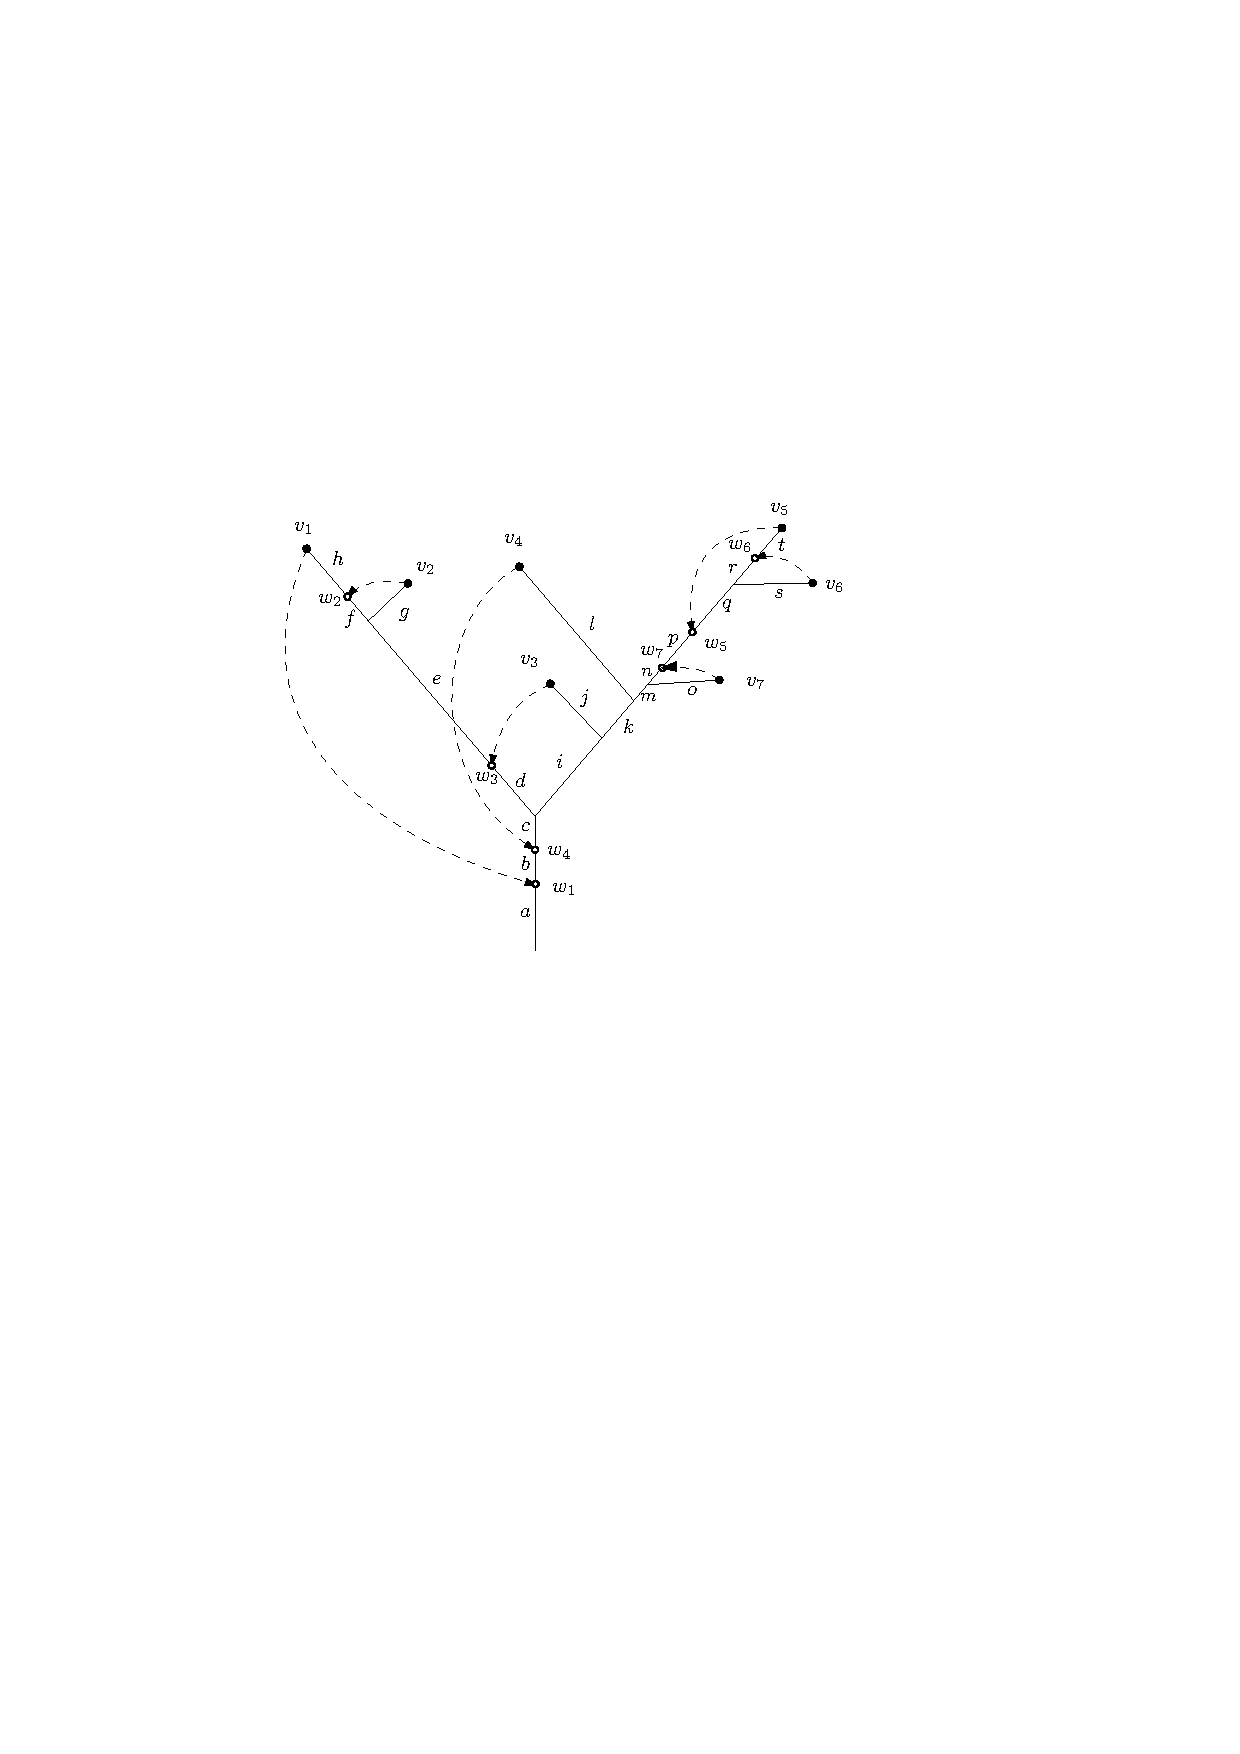
\includegraphics[width=0.8\linewidth]{Content/Pictures/out-componentwithcandidates.pdf}
    \caption{This is a subtree of an out-component spanned by the root of the out-component and the candidate tails $(v_1,\dots,v_7)$. Call the marked tree $T^{\mathrm{mk}}$. The heads of the candidates are denoted by $(w_1,\dots,w_7)$. }
\label{figure.extractSCCs1}
\end{subfigure}\\
\vspace{1.5em}
\begin{subfigure}{.8\textwidth}
  \centering
  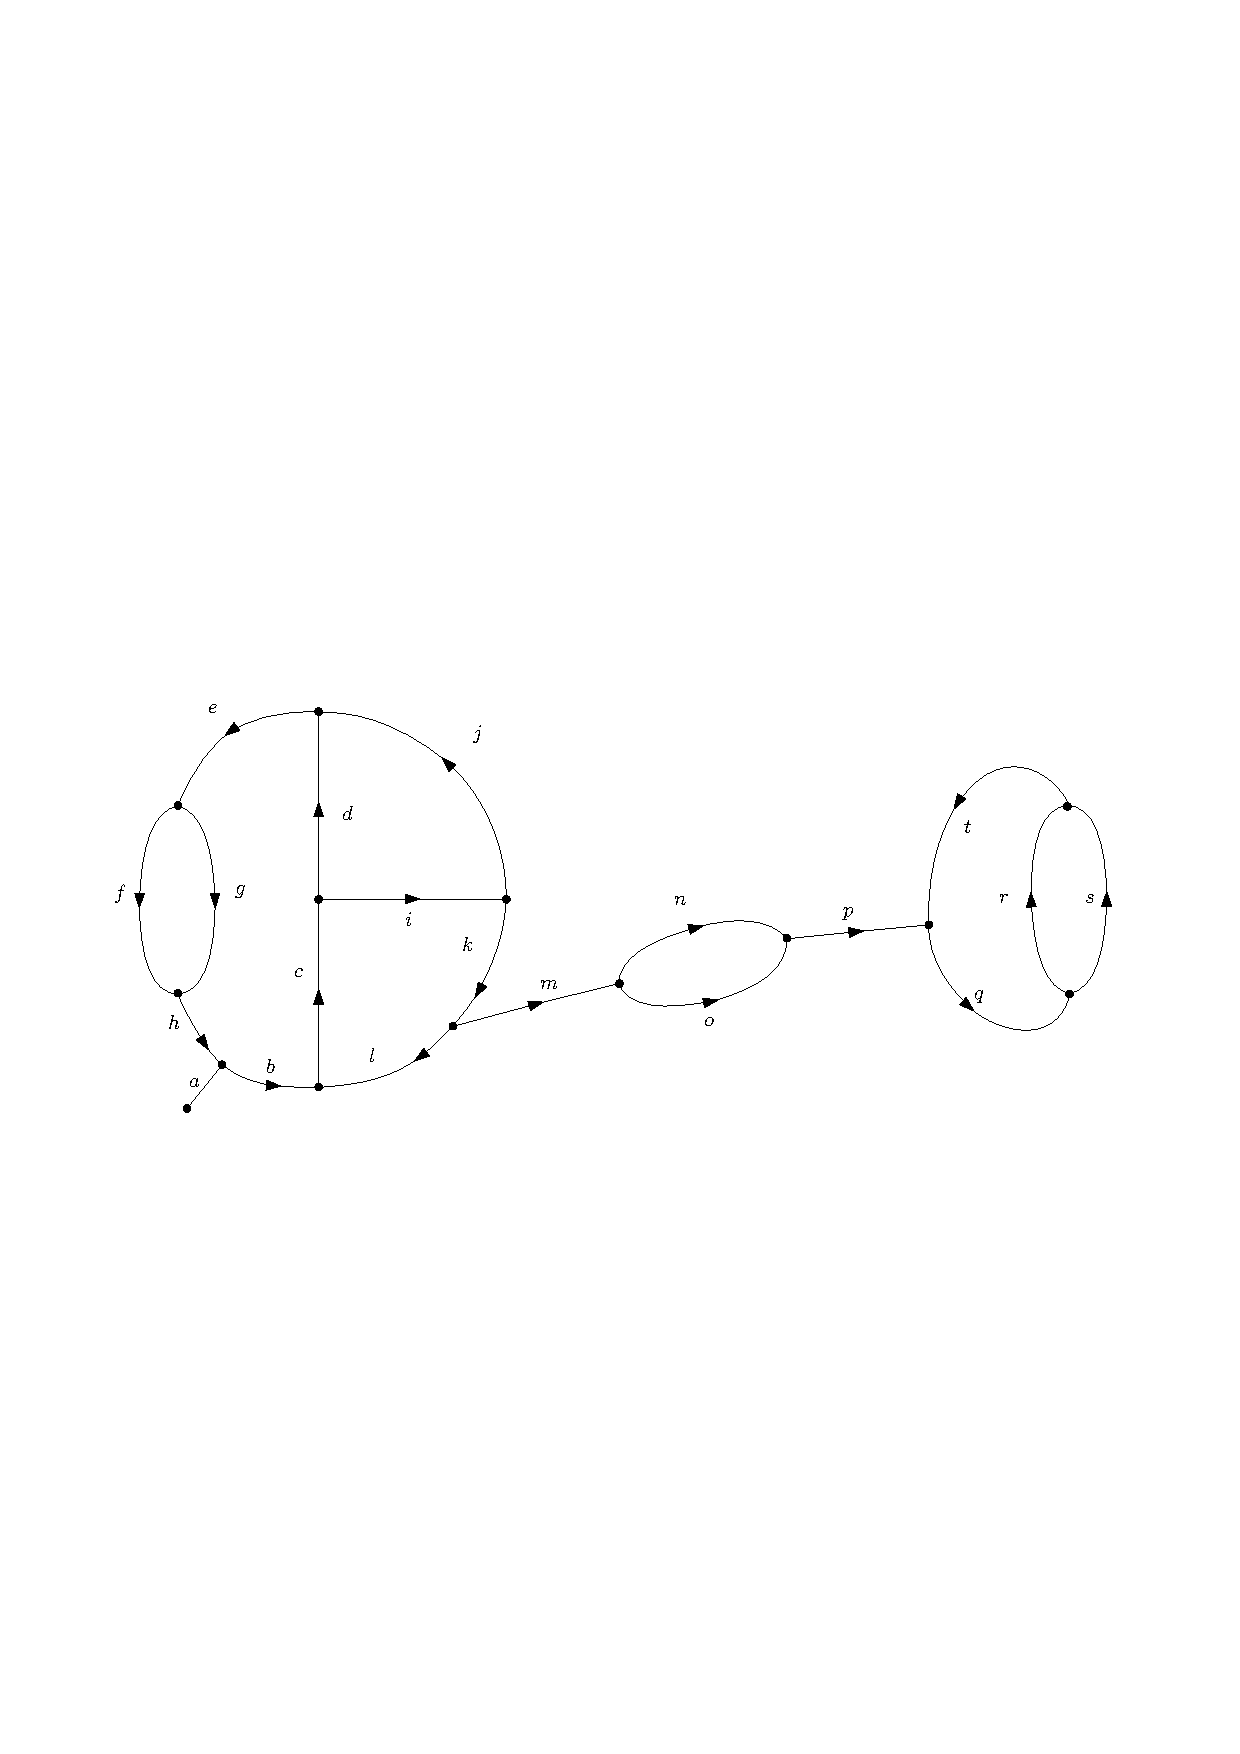
\includegraphics[width=0.9\linewidth]{Content/Pictures/identification.pdf}
  \caption{Identifying $v_i$ with $w_i$ for $i\in [7]$ gives $M$.}
  \label{figure.extractSCCs2}
\end{subfigure}\\
\vspace{1.5em}
\begin{subfigure}{.8\textwidth}
  \centering
  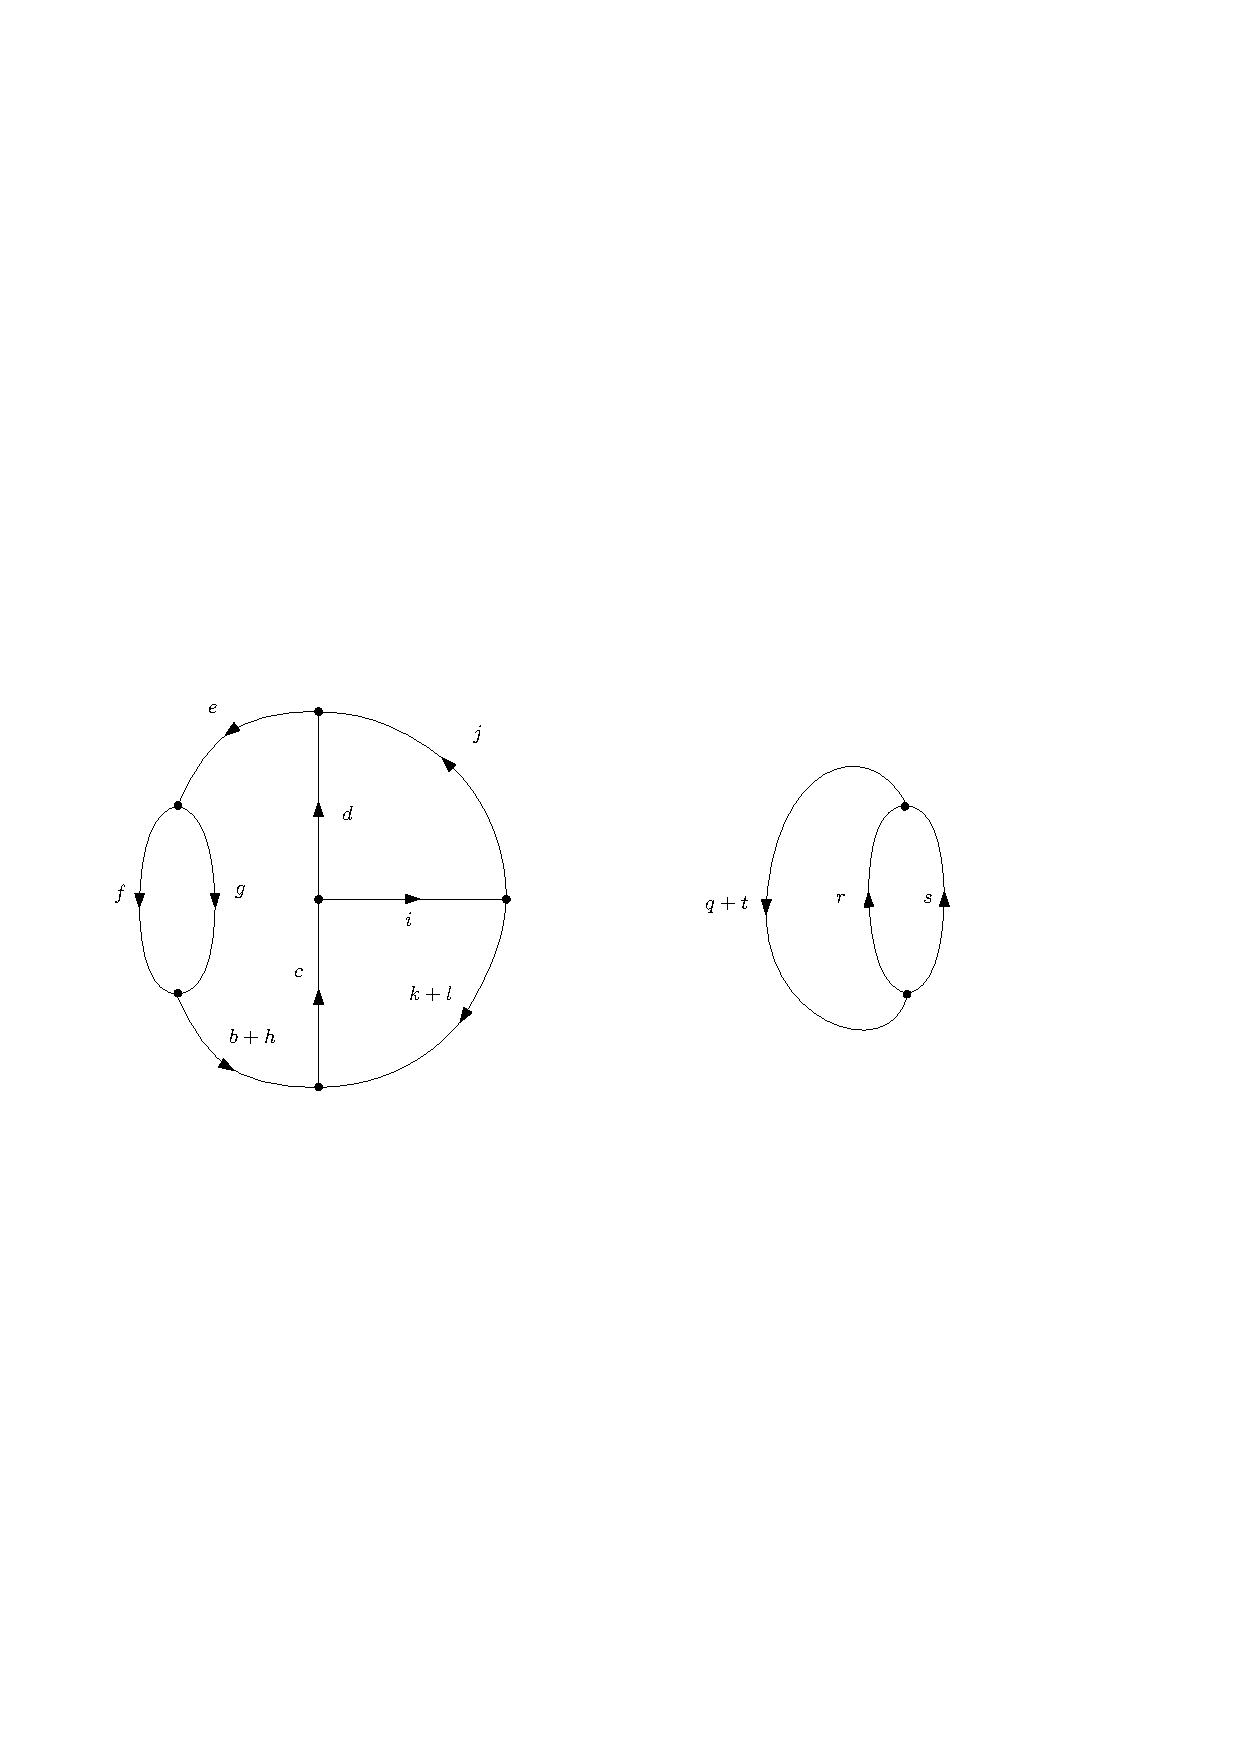
\includegraphics[width=0.9\linewidth]{Content/Pictures/cutting.pdf}
  \caption{We find the SCCs that are contained in $M$.}
  \label{figure.extractSCCs3}
\end{subfigure}

\caption{We illustrate the procedure to find the strongly connected components in a component of the out-forest after finding the candidates. Figures are created by Goldschmidt and Stephenson \cite{goldschmidtScalingLimitCritical2019}}
\end{figure}

\subsection{The continuum case}\label{subsec.limitobject}

We will define now define the continuous counterpart of the sampling procedure of the out-forest and the candidates. This is a modification of the procedure defined in Subsubsection 3.2.2 of \cite{goldschmidtScalingLimitCritical2019}. \\

\subsubsection{\texorpdfstring{$\R$}{R}-trees and their encoding}
The continuum analogue of discrete trees are given by $\R$-trees. A survey paper on $\R$-trees can be found in \myworries{insert Le Gall reference}. An $\R$-tree is a compact metric space $(\cT, d)$ such that for every $a, b \in \cT$ the following two properties hold:
\begin{enumerate}
    \item There exists a unique isometry $i_{a, b} : [0, d(a, b)] \to \cT$ such that $i_{a, b}(0) = a$ and $i_{a, b}(d(a, b)) = b$.
    \item If $q: [0, 1] \to \cT$ is any continuous map such that $q(0) = a$ and $q(1) = b$ then the image of $q$ is the same as the image of $i_{a, b}$.
\end{enumerate}
Let $\pathbtw{a, b}$ denote the image of $i_{a, b}$. This is the unique path between $a$ and $b$.

$\R$-trees are often encoded by continuous excursions which can be seen as a continuous analogue of the height function of a tree. Let $f: [0, \sigma] \to [0, \infty)$ be a continuous excursion, meaning $f$ is continuous, $f(0) = f(\sigma) = 0$ and $f(x) > 0$ for all $x \in (0, \sigma)$. Using $f$ we can define a pseudo-metric
\begin{equation*}
    d_f(x, y) = f(x) + f(y) - 2 \min_{s \in [x \wedge y, x \vee y]} f(s).
\end{equation*}
Using this we can define the quotient space
\begin{equation*}
    \cT_f = [0, \sigma] / \{d_f = 0\}.
\end{equation*}
The space $\cT_f$ equipped with the metric $d_f$ is the $\R$-tree encoded by the excursion $f$. Let $p_f: [0, \sigma] \to \cT_f$ be the natural projection function. Then $\cT_f$ inherits a distinguished root vertex $\rho = p(0) = p(\sigma)$.

\subsubsection{The limit object}\label{subsubsec.samplecontinuousobject}
Let $(B_t,t\geq 0)$ be a Brownian motion, and set $$\left(\hat{B}_t,t\geq 0\right)=\left(B_t-\frac{\sigma_{-+}+\nu_-}{2\sigma_+\mu}t^2,t\geq 0\right).$$ 
\begin{remark}
We note that the coefficient of the parabolic drift is negative. Indeed, the sign of the parabolic drift is the same as the sign of $\mu-\E[D^+(D^-)^2]$, and we note that
$$\frac{\E[(D^-)^2D^+]}{\E[D^+]}-\left(\frac{\E[D^+D^-]}{\E[D^+]}\right)^2=\frac{\E[(Z^+)^2]}{\mu}-1$$
is the variance of $D^-$ under the law of $\mathbf{D}$ size-biased by $D^+$, which is positive. Hence $\E[D^+(D^-)^2]/\mu\geq 1$, which shows that $(\hat{B}_t)_{t\geq 0}$ is a Brownian motion with a downwards parabolic drift.
\end{remark}
Define 
$$(\hat{R}_t,t\geq 0)= \left(\hat{B}_t-\inf\left\{\hat{B}_s: s\leq t\right\},t\geq 0\right).$$
Then, it is standard that $\left(\frac{2}{\sigma_+}\hat{R}_t,t\geq 0\right)$ is the height process corresponding to an $\R$-forest with \L ukasiewicz path $\left(\sigma_+\hat{B}_t,t\geq 0\right)$.  This fact also follows from the argument in Section \ref{sec.convoutforest}. Call this forest $(\hat{\cF}(t),t\geq 0)$. \\
Let $(A_t,t\geq 0)$ be a Cox process of intensity $$\frac{2(\sigma_{-+}+\nu_-)}{\sigma_+\mu^2} \hat{R}_t$$ at time $t$. Then, fix $T>0$, so that $A_T<\infty$ almost surely. For $i$ in $\left[A_T\right]$, set $X_i=\min\{t:A_T=i\}$. Define
\begin{align*}
L_i&=\inf\left\{t\geq 0:=\hat{B}_t=\inf\{\hat{B}_s:s\leq X_i\}\right\}\text{ for }i\in \left[A_T\right]\text{ and}\\
\Sigma_i&=\inf\left\{ t\geq 0: \inf\{\hat{B}_s:s\leq L_i+t\} < \inf\{\hat{B}_s:s\leq X_i\}\right\}\text{ for }i\in \left[A_T\right],
\end{align*}
so that for each $i$ in $\left[A_T\right]$, $\left(\frac{2}{\sigma_+}\hat{R}_t,t\in [L_i,L_i+\Sigma_i]\right)$ encodes the $\R$-tree in $(\hat{\cF}(t),t\geq 0)$ that contains $X_i$. For each element of $\{(L_i,\Sigma_i):i\in A_T\}$ we will sample the candidates in the $\R$-tree. Fix $i$, and set $(l,\sigma)=[L_i,\Sigma_i]$. Let $V_1=\inf\{s>0:A(s)=A(l)+1\}$, so that $l\leq V_1\leq l+\sigma$ by definition of $(l,\sigma)$. Let $\cT_l$ be the $R$-tree encoded by $\left(\frac{2}{\sigma_+}\hat{R}_t,t\in [l,l+\sigma]\right)$ and let $p_l:[l,l+\sigma]\to \cT_l$ be the projection onto $\cT_l$ given by the encoding. Set $$||\cT_l||=\sup\left\{\frac{2}{\sigma_+}\hat{R}_t,t\in [l,l+\sigma]\right\},$$
which we note is the height of $\cT_l$. \\
Suppose we have found candidates $\{V_1,\dots,V_m\}$. For $V_m\leq s\leq l+\sigma$, let $T^{\text{mk}}_s$ be the subtree of $\cT_l$ spanned by $p_l\left(\{l,V_1,\dots,V_m,s\}\right)$, and let $|T^{\text{mk}}_s|$ be its total length. Then, let $V_{m+1}$ be the first arrival time of a Poisson process on $[V_m,l+\sigma]$ of intensity $$\frac{\sigma_{-+}+\nu_-}{\mu^2}|T^{\text{mk}}_s|ds.$$ If the process does not contain a point, let $\{V_1,\dots,V_m\}$ be the candidates of $\cT_l$, and set $N=m$. Otherwise, we repeat the inductive step for $\{V_1,\dots,V_{m+1}\}.$ If the induction does not terminate, we set $N=\infty$.\\
We claim that $\P(N=\infty)=0$. Indeed, note that $V_m\leq s\leq V_{m+1}$ implies that  $|T^{\text{mk}}_s|<(m+1)||\cT_l||$. Therefore, 
$$\P\left(\left.N\geq l+1,V_{m+1}-V_m<t \right|N\geq l\right)\leq \P(E_{m+1}<t),$$
for $(E_{k},k\geq 1)$ a sequence of exponential random variables with respective rates $$\frac{\sigma_{-+}+\nu_-}{\mu^2}k||\cT_l||.$$ 
Then,
$$\P\left(N=\infty \right)=\P\left(N=\infty\text{ and }\sup\{c_i:i\in \N\}<l+\sigma\right)\leq \P\left(\sum_{i=2}^\infty E_k\leq l+\sigma-V_1\right).$$
However, $\sum_{i=2}^\infty E_k=\infty$ a.s., because the harmonic series diverges, so, indeed, $\P\left(N<\infty \right)=1$. \\
Finally, for $1\leq i \leq N$, let the head corresponding to $V_i$, which we call $W_i$, be a uniform pick from the length measure on $T^{\text{mk}}_{V_i}$. \\
Let $T^{\text{mk}}_l$ be the subtree of $\cT^{l}$ spanned by $\{l,V_1,\dots,V_N\}$. Then, in $T^{\text{mk}}_{l}$, set $V_i\sim W_i$ for each $1\leq i\leq N$, and set $\cM_{l}:=T^{\text{mk}}_{l}/\sim$. View $\cM_{l}$ as an element of $\vec{\cG}$ in the natural way, and call it $M_l$. To be precise,  let the vertex set of $M_l$ consist of $l$, $W_i$ for $i\leq N$, and the branch points $V_i\wedge V_j$ for $i\neq j\leq N$. The directions are inherited from $\cT^l$, by considering all edges directed away from the root. Remove all edges that do not lie in a strongly connected component of $M_{l}$ and delete any isolated vertices that are thus created. Then, for any vertices of degree $2$, merge the neighbouring edges and sum their lengths. This creates a collection $\cC_l$ of strongly connected MDMs. Doing this for each $(l,\sigma)\in \{[L_i,\Sigma_i]\}$ yields the collection of strongly connected MDMs $\cC$ that has the law of the limit in Theorem \ref{thm.main}.

\subsubsection{Properties of the limit object}
We note that the limit object is encoded by $3$ parameters: the real forest is encoded by a Brownian motion with variance $\sigma_+^2$ and parabolic drift with coefficient $-(\sigma_{-+}+\nu_-)/(2\mu)$, and the identifications are a Cox process with intensity $(\sigma_{-+}+\nu_-)/\mu^2$ on the length measure of the subtree spanned by the previously found candidates and the currently explored point as described in \ref{subsubsec.samplecontinuousobject}. The limit object that is studied in \cite{goldschmidtScalingLimitCritical2019} corresponding to $\lambda=0$ (i.e. at criticality) is equal to our limit object in the case $\sigma_+^2=1$, $-(\sigma_{-+}+\nu_-)/(2\mu)=-1/2$, and $(\sigma_{-+}+\nu_-)/(\mu^2)=1$. Note that these three conditions are satisfied if we let $D^-$ and $D^-$ be independent $\operatorname{Poisson}(1)$ random variables. In \cite{goldschmidtScalingLimitCritical2019}, some properties of the limit object corresponding to these specific parameters are shown. A quick check shows that the proofs do not depend on the values of the parameters, so we deduce that the properties also hold for our limit object. Let $\cM:=\bigcup_{L_i}\cM_{L_i}$.

\begin{corollary}
\begin{enumerate}
    \item The number of complex connected components of $\cM$ has finite expectation.
    \item The number of loops of $\cM$ is a.s. finite.
\end{enumerate}
\end{corollary}
\begin{proof}
The proof is analogous to the proof of Theorem 4.5 in \cite{goldschmidtScalingLimitCritical2019}.
\end{proof}
\begin{corollary}\label{cor.allengthsaredifferent}
The strongly connected components of $\cM$ all have different lengths almost surely.
\end{corollary}
\begin{proof}
The proof is analogous to the proof of Proposition 4.6 in \cite{goldschmidtScalingLimitCritical2019}.
\end{proof}
Write $\cC$ for the strongly connected components of $\cM$ and $\mathbf{C}_l$ for those of $\cM_l$, in decreasing order of length, with $\cM_l$ as defined in Subsubsection  \ref{subsubsec.samplecontinuousobject}. Write $\cC_{\text{cplx}}$ for the list of complex components of $\cC$ in decreasing order of length. For sequences $(K_1,\dots, K_j)$ and $(J_1,\dots,J_k)$ of directed multigraphs, write $(J_1,\dots,J_k)\equiv(K_1,\dots, K_j)$ if $j=k$ and $J_i$ is isomorphic to $K_i$ for each $i\leq j$. Extend this notation naturally to the case where one or both of the sequences has edge lengths by ignoring the edge lengths. 
\begin{corollary}
Let $K_1,\dots, K_j$ be a finite sequence consisting of $3$-regular strongly connected directed multigraphs or loops. We have 
$$\P\left[\cC_l\equiv(K_1,\dots, K_j)\right]>0.$$
Assuming that $K_1,\dots, K_j$ are all complex, we also have that 
$$\P\left[ \cC_{\text{cplx}}\equiv(K_1,\dots, K_j)\right]>0.$$
Let $(e_i,1\leq i \leq K)$ be an arbitrary ordering of the edges of $K_1,\dots, K_j$. Then, conditionally on $\cC_l\equiv(K_1,\dots, K_j)$, (resp. $\cC_{\text{cplx}}\equiv(K_1,\dots, K_j)$), $\cC_l$ (resp. $\cC_{\text{cplx}}$) gives lengths $(\ell(e_i),1\leq i \leq K)$ to these edges, and their joint distribution has full support in 
$$\left\{\mathbf{x}=(x_1,\dots, x_K)\in \R_+^K:\forall 1\leq i\leq k-1, \sum_{j:e_j\in E(K_i)}x_j \geq \sum_{j:e_j\in E(K_{i+1})}x_j\right\}.$$
\end{corollary}
\begin{proof}
The proof is analogous to the proof of Theorem 6.1 in \cite{goldschmidtScalingLimitCritical2019}.
\end{proof}

